\chapter{Methods}
In this chapter the methods needed to create a parametric model and  a mapping between parametric models are introduced and explained. First off, the data gathering and preprocessing are outlined. Multiple variants of the parametric model are discussed. Different learning approaches for the mapping are reviewed. Lastly, a character editor is presented that is used to generate data for a parametric model.

\section{Data Acquisition and Preprocessing}
Optimally it would be necessary to have a large data set of images of women before and after breast enhancement surgery, where the patients pose topless. It is very unlikely though that such a database exists, due to the fact that having breast surgery is a very personal topic and people generally don't enjoy posing naked. Therefore the images used were downloaded from a website\footnote{https://my.crisalix.com/} that offered to simulate various plastic surgical procedures including breast enhancement. For each user a 3D model of their torse was displayed side by side with different enhancements varying in size. Each model was made up of a sequence of 24 images displaying the torse from different angles. This dataset fit the requirements nicely as images are available for \textit{before} and \textit{after}, except the \textit{after} is generated and based on their model. Additionally, each after image sequence had a short label, usually describing how much silicon was added, that was also saved for further evaluation. In total 2'937 examples were retrieved and preprocessed. This dataset included images from 748 subjects of which each one was comprised of one \textit{before} and at least one \textit{after} image sequence.\\

In a next step these image sequences needed to be transformed into point clouds. This was done using a general-purpose Structure-from-Motion (SfM) \cite{schoenberger2016sfm} and Multi-View Stereo (MVS) \cite{schoenberger2016mvs} pipeline called COLMAP. This generated point clouds spanning from 5'000 to 15'000 points. Some of the images needed to be discarded, due to the fact that SfM created a point cloud with less than 1'000 points or the point clouds had holes, such that certain areas had no points and were not defined at all. The remaining point clouds were cleaned using a C++ implementation by Biland \cite{Biland17} that removed white points around the point clouds.

The mapping required to have one set of point clouds of \textit{before} examples and the corresponding\footnote{Corresponding meaning, based on the same subject.} \textit{after} examples. Therefore the data was split into sets of \textit{before} and after point clouds. Additionally, to create a better mapping, only the \textit{after} examples that were labelled "350" were included. This resulted in 57 examples in the \textit{before} and 57 in the \textit{after} set. All of these point clouds were further processed in a MATLAB implementation by Biland \cite{Biland17} to generate mesh files.

\subsection{Alignment}
\label{align}
Eventhough the meshes were aligned in the MATLAB implementation by Biland \cite{Biland17} in a general fashion, each corresponding \textit{before} and \textit{after} should be pairwise aligned to avoid that the mapping also learns rotations. This was achieved by using an implementation of Horn's method \cite{horn1987closed}. Given two sets of vertices, Horn's method computes the translation, rotation and possibly scale change from one set to the other. As it is expected that for the same subject, only points defining the breasts should vary from before to after, only a subset of vertices should be used. The points used in the alignment can be seen in figure \ref{fig:alignment}.

\begin{figure}[h]
\centering
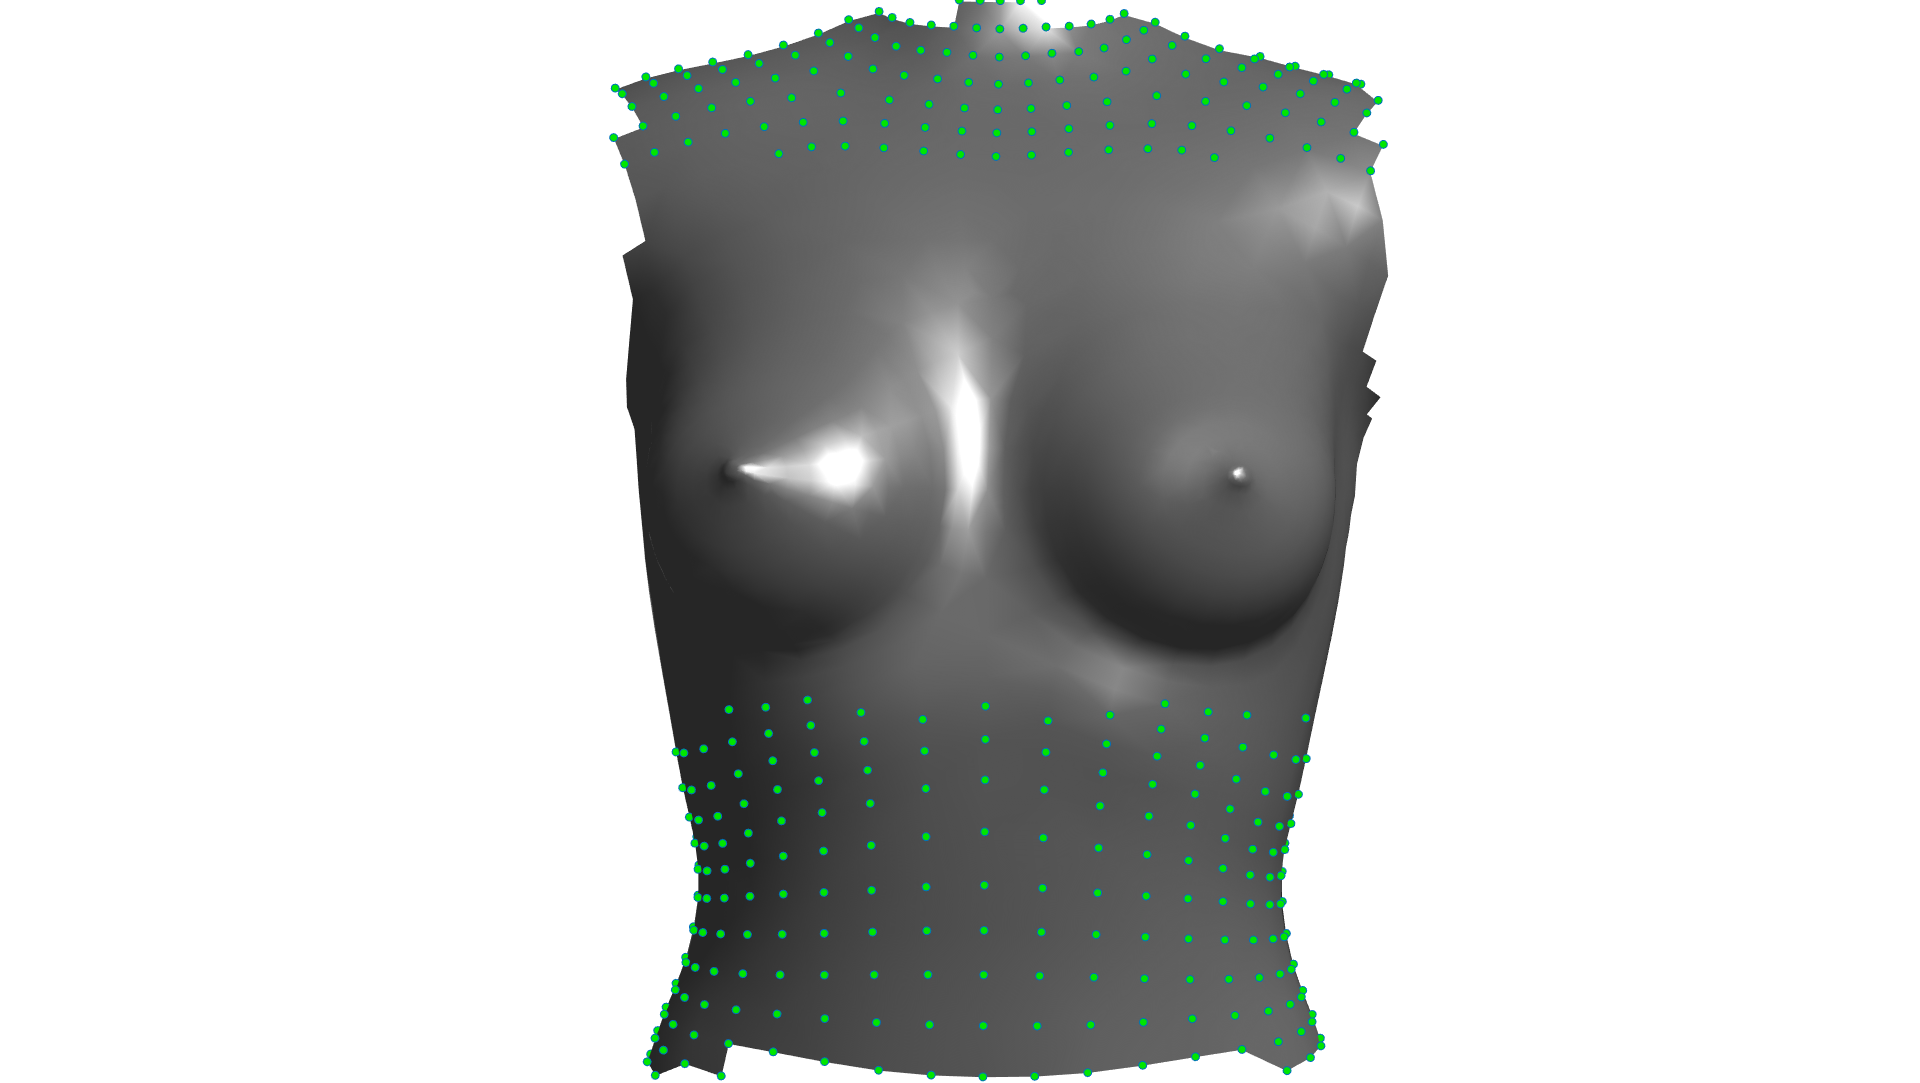
\includegraphics[width=0.75\textwidth]{figures/alignment}
\caption{The mesh is depicted as the grey surface. The points drawn in green are used for the alignment.}
\label{fig:alignment}
\end{figure}

\section{Parametric Model from Meshes}
\label{paramModel}
In this section it is described how a parametric model is obtained using principle component analysis (PCA). Given $n$ meshes $m_i \in \mathbb{R}^{k \times 3}$, where $k$ describes the amound of vertices $m$ has, each mesh needs to be transformed to be of shape $\mathbb{R}^{1 \times 3k}$. Then, all transformed meshes are stacked into a matrix $M \in \mathbb{R}^{n \times 3k}$. As the differences over each column isn't significant, the mean $\bar{m}$ of the matrix $M$ is subtracted from each row of $M$.
\begin{gather}
\mathbf{A} :=
\begin{bmatrix}
 m_1' - \bar{m} \\
 m_2' - \bar{m} \\
 \vdots \\
 m_n' - \bar{m}
\end{bmatrix}
\in \mathbb{R}^{n \times 3k}
\end{gather}

Next, PCA is run with matrix $A$ as the input. PCA is able to reduce the dimensionality of the data while retaining most of the information from the initial data set. This is achieved by finding orthogonal basis vectors, where the first basis vector is responsible for the largest variance in the data. The second basis vector needs to be orthogonal to the first and is responsible for the second largest variance of the data. This holds for each following basis vector. These basis vectors in PCA are also known as principle components.

The output of the PCA function is:

\begin{gather}
\mathbf{coeff} :=
\begin{bmatrix}
 c_1&c_2&\cdots&c_{n-1}
\end{bmatrix}
\in \mathbb{R}^{3k \times n-1}
\end{gather}
\begin{gather}
\mathbf{score} :=
\begin{bmatrix}
s_1&s_2&\cdots&s_{n-1}
\end{bmatrix}
\in \mathbb{R}^{n \times n-1}
\end{gather}

where coefficient $c_i$ is the $i$-th principle component and score $s_i$ is the $i$-th parameter vector corresponding to the $i$-th input. Therefore the input data can be reproduced by computing $\mathbf{A = score \times {coeff}^T}$. Instead of using all $n-1$ coefficients it is possible to only use the first $\mathbf{q}$ coefficients resulting in an approximation of the space. The parameters $\mathbf{p_{q,new}}$ for a new input mesh $m_{new}$ can be easily computed for $\mathbf{q}$ coefficients by first reshaping the mesh to be of the form $\mathbb{R}^{3k \times 1}$ and subtracting the mean $\bar{m}$. This is done the same way as above, adding an additional step to transpose. Then the pseudoinverse of $\mathbf{coeff_{(q)}}$ is multiplied from the left to compute the corresponding parameters $\mathbf{p_{q,new}}$:
\begin{gather}
\mathbf{p_{q,new}} = \mathbf{coeff^+_{(q)}} \cdot (m_{new}' - \bar{m})^T  \text{  where }
\mathbf{coeff_{(q)}} :=
\begin{bmatrix}
 c_1&c_2&\cdots&c_{q}
\end{bmatrix}
\in \mathbb{R}^{3k \times q}
\end{gather}

In this example the parametric model is based on the vertices of the mesh. In the next subsections, two other variants are explored and explained.
\subsection{Face Deformations}
\label{faceDeform}
Instead of defining a mesh by its vertices, it is possible to describe it by the deformations of the faces. This is done by defining one source mesh and computing how each face is deformed. One way to quantify a deformation of a face was described by Sumner \cite{sumner2004deformation}, where the idea was to transfer triangle deformations between similar meshes. First, a new vertex needs to be computed such that an affine transformation can be determined. The fourth vertex is defined as follows:
\begin{gather}
  \mathbf{v_4} = \mathbf{v_1} + (\mathbf{v_2} - \mathbf{v_1})\cross(\mathbf{v_3}-\mathbf{v_1})/\sqrt{\lvert(\mathbf{v_2}-\mathbf{v_1})\cross(\mathbf{v_3}-\mathbf{v_1})\rvert} \label{normalequation}
\end{gather}
%% Add image of triangle with a point added along the normal to describe what is happening up here
\begin{figure}[h]
\centering
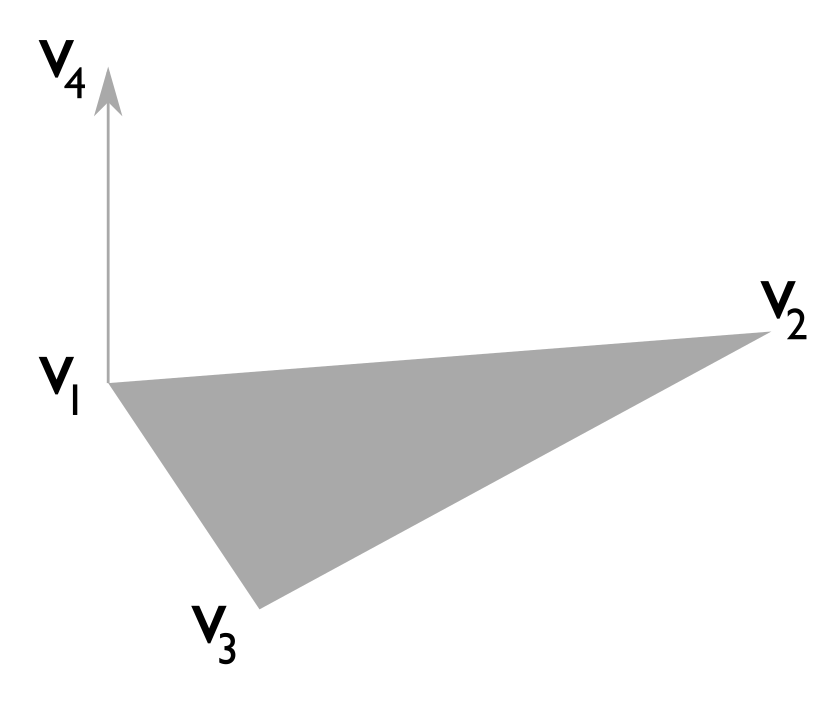
\includegraphics[width=0.4\textwidth]{figures/normal}
\caption{A vertex is added to the triangle that lies in the direction of the normal.}
\label{fig:normal}
\end{figure}

The crossproduct is scaled by the reciprocal of the square root of its length, to keep the distance proportional to the length of the traingle edges. See figure \ref{fig:normal} for a visualization of adding a vertex on the normal.
Given both faces with one additional vertex, the following equations can be posed:
\begin{gather}
 \mathbf{Q}\mathbf{v_i}+\mathbf{d} = \mathbf{\tilde{v}_i}, \mathbf{i} \in \mathbf{1} \dotsc \mathbf{4}
\end{gather}
where $\mathbf{Q} \in \mathbb{R}^{3 \cross 3}$ and translation vector $\mathbf{d}$ describe the affine transformation. By subtracting the first equation from the following three equations and rewriting the resulting system in matrix form, the problem can be defined as $\mathbf{Q}\mathbf{V}=\mathbf{\tilde{V}}$ where
\begin{gather}
  \mathbf{V} =
  \begin{bmatrix}
   \mathbf{v_2} - \mathbf{v_1}&\mathbf{v_2} - \mathbf{v_1}&\mathbf{v_2} - \mathbf{v_1}
  \end{bmatrix} \\
  \mathbf{\tilde{V}} =
  \begin{bmatrix}
   \mathbf{\mathbf{v}_2} - \mathbf{\mathbf{v}_1}&\mathbf{\mathbf{v}_2} - \mathbf{\mathbf{v}_1}&\mathbf{\mathbf{v}_2} - \mathbf{\mathbf{v}_1}
  \end{bmatrix}
\end{gather}
The closed form expression for $\mathbf{Q}$ is defined as
\begin{gather}
  \mathbf{Q}=\mathbf{\tilde{V}}\mathbf{V}^{-1}
\end{gather}
To fully describe a mesh, this $\mathbf{Q}$ matrix needs to be computed for each face of the mesh. Finally, the mesh is represented by $\mathbf{D} \in \mathbb{R}^{3 \times 3h}$ where $\mathbf{h}$ is the number of faces the mesh has. To be able to run PCA, each mesh needs to be reshaped to be of form $\mathbf{D'} \in \mathbb{R}^{1 \times 9h}$ and the rest of the process is the same as above in section \ref{paramModel}.

\subsection{Point Normals}
This method is very much similar to one described in section \ref{paramModel}. In addition to the vertices of the mesh, one vertex per face is computed as described in equation \ref{normalequation} and added to the list of vertices of the mesh. Therefore the mesh matrix will be of form $\mathbb{R}^{k+h \times 3}$ where $\mathbf{k}$ is the number of original vertices and $\mathbf{h}$ is the number of faces of the mesh.

\section{Mapping}
The following segment describes how a mapping can be computed in a linear or a non-linear way. The data available is the parameters returned by both the parametric models for the before and after examples. The matrices of the data are
\begin{gather}
  \mathbf{P_{before}} =
  \begin{bmatrix}
    \mathbf{p_{b,1}} \\
    \mathbf{p_{b,2}}  \\
    \vdots \\
    \mathbf{p_{b,n}}
  \end{bmatrix}
  \in \mathbb{R}^{n \cross n-1},
  \mathbf{P_{after}} =
  \begin{bmatrix}
    \mathbf{p_{a,1}} \\
    \mathbf{p_{a,2}} \\
    \vdots \\
    \mathbf{p_{a,n}}
  \end{bmatrix}
  \in \mathbb{R}^{n \cross n-1}
\end{gather}
where each parameter pair $(\mathbf{p_{b,i}}, \mathbf{p_{a,i}})\ \forall i$ is related, as the after was generated from the before.

\subsection{Linear Method}
The first method used, was the linear system solver by MATLAB (also known as backslash \ solver) that solved the equation
\begin{gather}
  \mathbf{P_{before}} \cdot \mathbf{M_{linear}} = \mathbf{P_{after}}
  \text{ where } M_{linear} \in \mathbb{R}^{n-1 \times n-1}.
\end{gather}
It is clear that an explicit linear transformation could be found for each parameter pair, but the goal is to have one mapping that works for each parameter pair. This is also known as linear regression. One basic example in linear regression is the task of fitting a line to a point cloud. As all the points of the point cloud do not lie on one line, it isn't possible to define a straight line. Therefore a line is sought after, such that all points are as close as possible on average. This is depicted in figure \ref{fig:linReg}.

\begin{figure}[h]
\centering
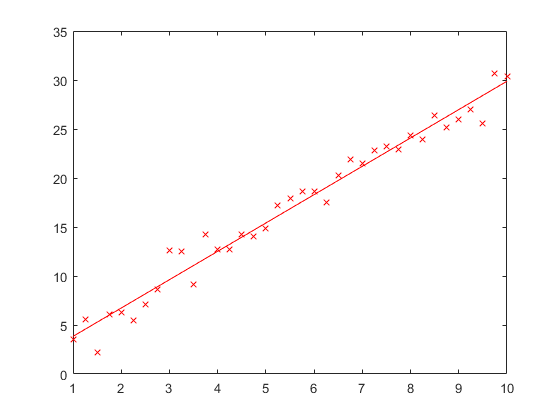
\includegraphics[width=0.7\textwidth]{figures/linReg}
\caption{Fitting a line to a point cloud using linear least-squares.}
\label{fig:linReg}
\end{figure}

\subsection{Non-Linear Variants}
This section deals with non-linear methods to solve the regression problem described above. All the methods used are part of the scikit-learn library \cite{scikit-learn}. It is common in a machine learning setting to split data into two sets. One set is used to train the model and the other is used to evaluate how well the method does on data, that was not part of the first set. Both data sets should be drawn from the same distribution. This is necessary because the model shouldn't be penalized for performing badly on problems it didn't encounter in the training phase.\\
During the training phase it is standard to run grid search. Grid search varies the parameters of the model to find the best set of parameters for a specific task. It needs to be considered that grid search can lead to overfitting, this occurs when the error on the training set is reduced at the cost of increasing the test error. This can be avoided by adding regularization terms or by running grid search along with cross-validation.
\subsubsection{Decision Tree}
\label{sec:dt}
One category of machine learning approaches is based on so called decision trees (DT). A decision tree uses a tree-like approach, where nodes of the tree are defined to split the data set into subsets corresponding to groups. As an example, the goal is to have a model that can predict the weight of a person, based on height, daily activity and daily calorie intake as features. Using a decision tree, the value of height could split the data set, as taller people tend to be heavier than small people. This is done over all features until the complete data set is divided into smaller subsets. Leafs make up the end of a decision tree. Each leaf has a certain value connected to it, in the case mentioned before it would be a certain weight range or value. \\
When the weight of a new person would need to be predicted, one would follow the tree from top to bottom until a leaf was met. The corresponding weight value of the leaf would be equal to the prediction the model returns. An example of a decision tree can be seen in figure \ref{fig:dtdiag}.

\begin{figure}[h]
\centering
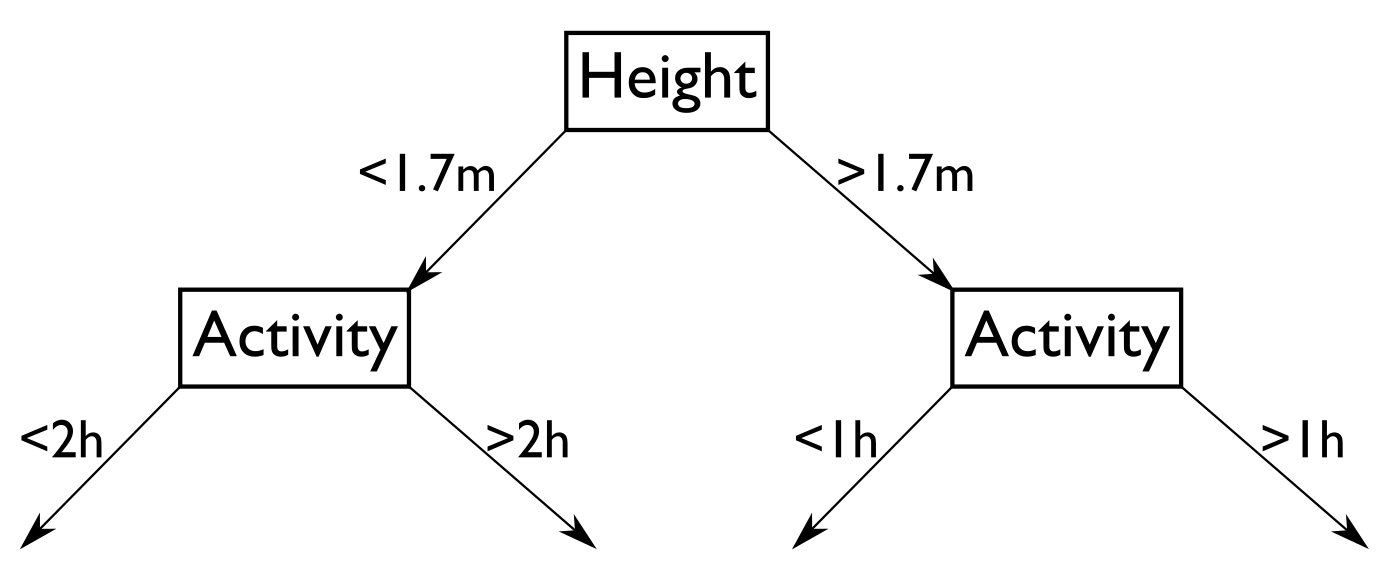
\includegraphics[width=0.75\textwidth]{figures/dtdiag}
\caption{Example of a decision tree following example of section \ref{sec:dt}}
\label{fig:dtdiag}
\end{figure}

\subsubsection{Random Forest}
The random forest (RF) regressor is also a tree-like approach similar to the decision tree. The main difference is that the decision tree considers all features when splitting and thus can be prone to overfitting. Random forest chooses features at random and builds decision trees based on those features. This is done for multiple trees until all subtrees are combined.

\subsubsection{Multilayer Perceptron}
The multilayer perceptron (MLP) is a type of neural network. It uses a feedforward approach to propagate information through the network. MLP have at least three layers where the first layer is the input layer and the last layer is the output layer. Each layer is made up of neurons, that receive information from the previous layer, apply some operation followed by an activation function and pass the result on to the next layer. These activations can either be linear or non-linear. It doesn't make sense to have multiple intermediate layers with linear activation functions, as each linear combination of linear functions, can be described one other linear function. \\
Each layer is made up of multiple neurons, each with their own weights and biases, and an activation function. All weights and biases are initialized at random. In the training phase a technique known as backpropagation is applied. Given an example, input and outcome, the input data is passed through all the layers. The resulting output is compared to the actual outcome. Given the difference between the two values, weights and biases are modified to reduce the difference, starting from the output layer, moving back through the hidden layers up to the input layer. A basic scheme of a MLP is shown in figure \ref{fig:mlpdiag}.

\begin{figure}[h]
\centering
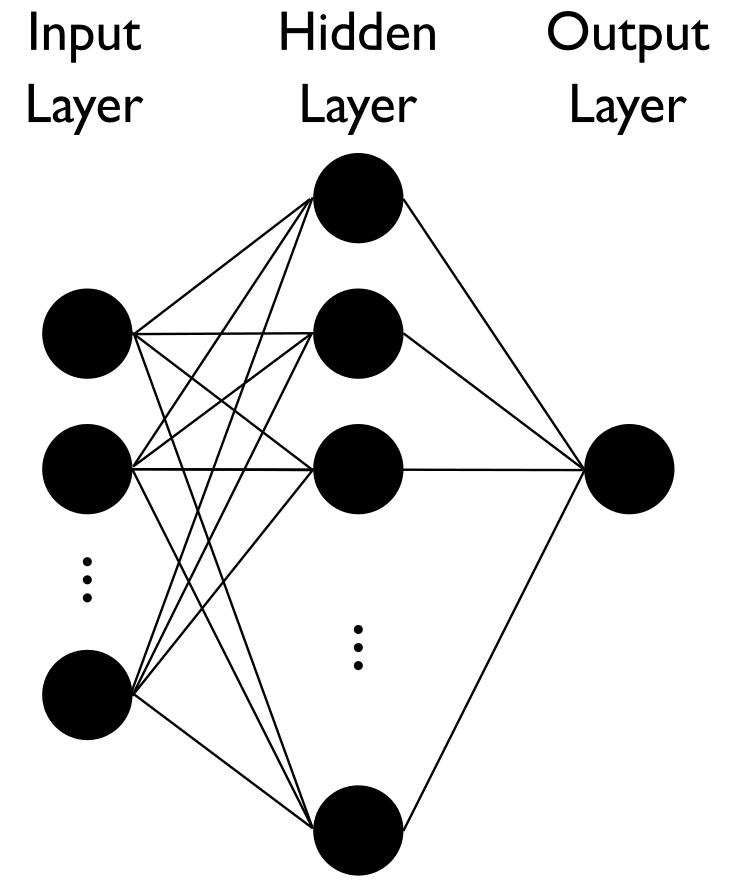
\includegraphics[width=0.3\textwidth]{figures/mlpdiag}
\caption{Scheme of a multilayer perceptron for regression.}
\label{fig:mlpdiag}
\end{figure}


\section{Parametric Model from Editor}
In all of the previous sections the parametric model was based off of real world data. In this section the same procedure is done as in section \ref{paramModel}, except that the meshes used for PCA were generated by software called MakeHuman \footnote{http://www.makehumancommunity.org/}. MakeHuman is a free and open source character modelling tool. It starts out with a gender neutral base mesh that can be modelled by varying sliders. These sliders apply linear interpolations to the base mesh between the extreme positions.\\
There are over 40 sliders in MakeHuman and the sliders are categorized by what areas of the body they modify. The graphical user interface of MakeHuman can be seen in figure \ref{fig:mhgui}. Using the scripting feature in MakeHuman multiple meshes could be generated, exported and later imported into MATLAB.

\begin{figure}[h]
\centering
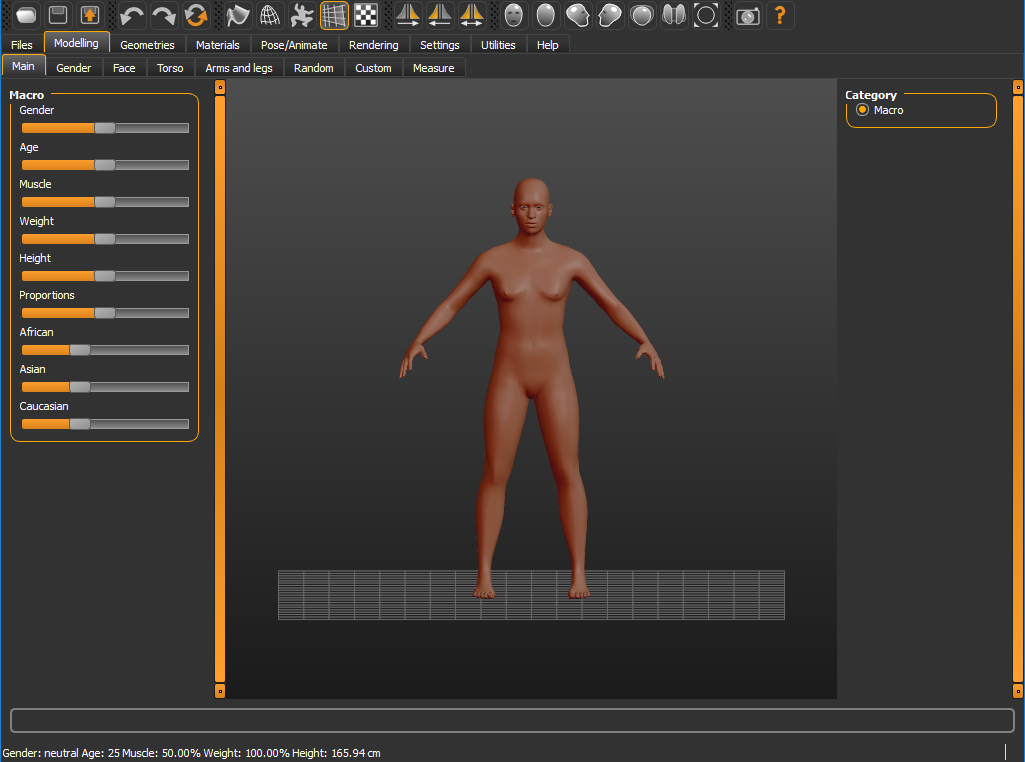
\includegraphics[width=1\textwidth]{figures/mhgui}
\caption{Graphical user interface of MakeHuman.}
\label{fig:mhgui}
\end{figure}

\section{Fitting parametric models to point clouds}
\label{fitModel}
Given a parametric model, it is possible to create a large diversity of possible outputs by varying the parameters. But finding the specific parameters for a new point cloud is a non-linear optimization problem. Therefore a C++ implementation by Biland \cite{Biland17}, using an open source C++ library for optimization problems called the Ceres solver \cite{ceres-solver}, was slightly modified and used. This implementation allows to fit a parametric model to a point cloud given a few keypoints of the point cloud.\\

In a first step the keypoints are used to find the parameters of translation, rotation and scaling. Afterwards a select number of points are chosen as correspondences between the model and the point cloud. Iteratively this implementation tries to minimize the distance between all the correspondences by varying the parameters of the model. Additionally, constraints are applied to the values the parameters are allowed to take. This prevents one parameter becoming too large and also possibly forcing the model to use multiple parameters than to rely on a single parameter. After a certain number of iterative steps has been reached, a certain threshold in accuracy is passed or the change in parameters is vanishingly small, the resulting mesh and parameters are returned.
